\subsection{Wrapper Generation}
The wrappers described in Section \ref{ld_preload_implementation} are uniformly structured: they contain one method, the signature of which is identical to that of the overridden call. Furthermore, nothing specific about the call's implementation is necessary for generating the wrapper. Thus, wrappers are good candidates for automatic code generation by inspection of the appropriate header files. For example, by examining the \texttt{stdlib.h} file and knowing one piece of information from the \texttt{MALLOC(3)} \texttt{man} page, we can completely construct the wrapper (Figure \ref{fig:codegen}).

\begin{figure}[h!]
\centering
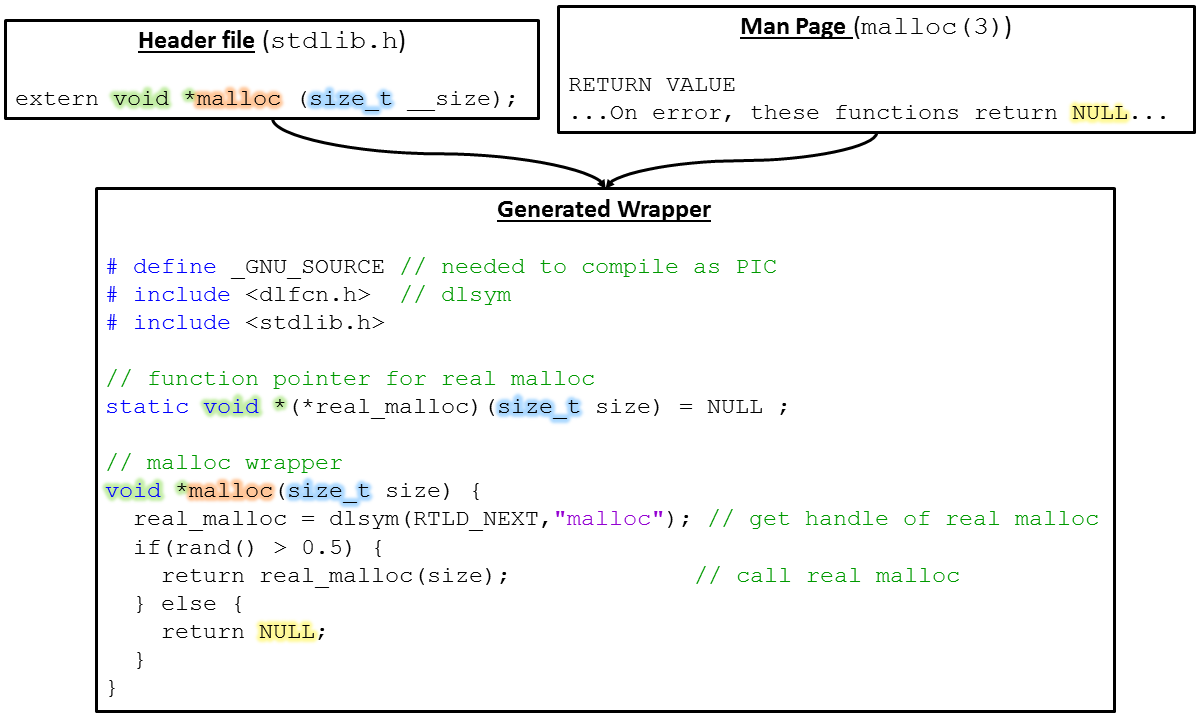
\includegraphics[width=0.8\textwidth]{codegen_figure}
\caption{Generation of wrappers is possible by parsing the abstract syntax tree of the appropriate header file and manually annotating the error value to be returned.}
\label{fig:codegen}
\end{figure}

We developed an input file which contained the call name, (error) return value, \texttt{errno} (if applicable), and the header file to be included in the wrapper (usually given at the top of the \texttt{man} page). Our script parsed this input file and generated the appropriate wrappers. The script uses the \texttt{pycparser} Python module \cite{pycparser} to traverse the abstract syntax tree derived from the header file.

This technique has several benefits, the primary one being that it reduces development time when wanting to make small changes to all of the wrappers. For example, after starting with a wrapper that simply returns the value of the real call using \texttt{dlsym}, we want to add a ``coin flip'', which simply determines at random whether to return the correct value or the error value. It is trivial to do this via code generation, by simply adding a few lines to the script and re-running it to update all of the downstream wrappers.

We are unsure whether the added development cost of this approach outweighs the potential speedup in development time. It is true that the wrapper files are only infrequently modified, however when dealing with almost 20 wrappers, it becomes increasingly tedious to make changes in a manual way. At the least, we hope that these techniques are useful for others in the testing community.